
%%%%%%%%%%%%%%%%%%
%%%%%%%%%%%%%%%%%%
\begin{frame}
\shiftedframetitle{5. Results}
%\vspace{-0.5cm}
%{\large $2D$ SWE - $2D$ SWE \textbf{\myTUMdarkblue{Unidirectional}}}\\
%Case: Radial dam break, no bathymetry
%\begin{textblock*}{1cm}(17cm,1pt) % {block width} (coords)
%%\begin{figure}
%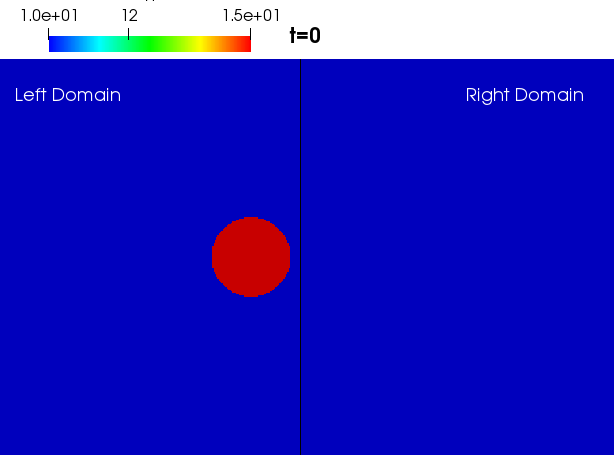
\includegraphics[scale=0.22]{./Resources/Images/unidirectional0_g_0.png}
%%\caption{sadf}
%%\end{figure}
%\end{textblock*}
%
%\begin{figure}[htp]
%\centering
%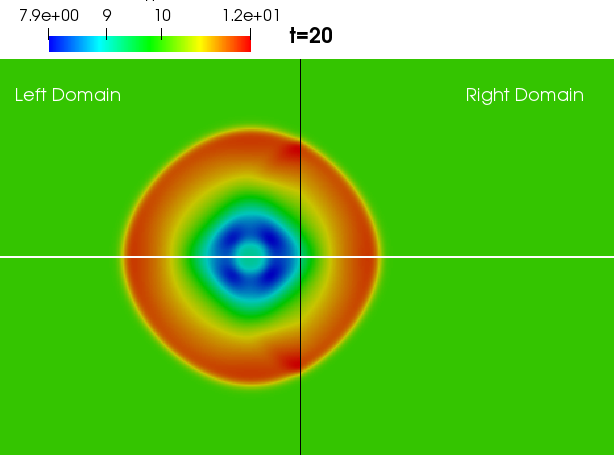
\includegraphics[width=.25\textwidth]{./Resources/Images/unidirectional20_g_0.png}\hfill
%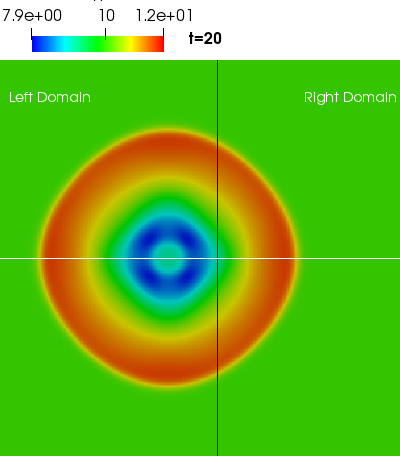
\includegraphics[width=.25\textwidth]{./Resources/Images/unidirectional20_g_bueno.png}\hfill
%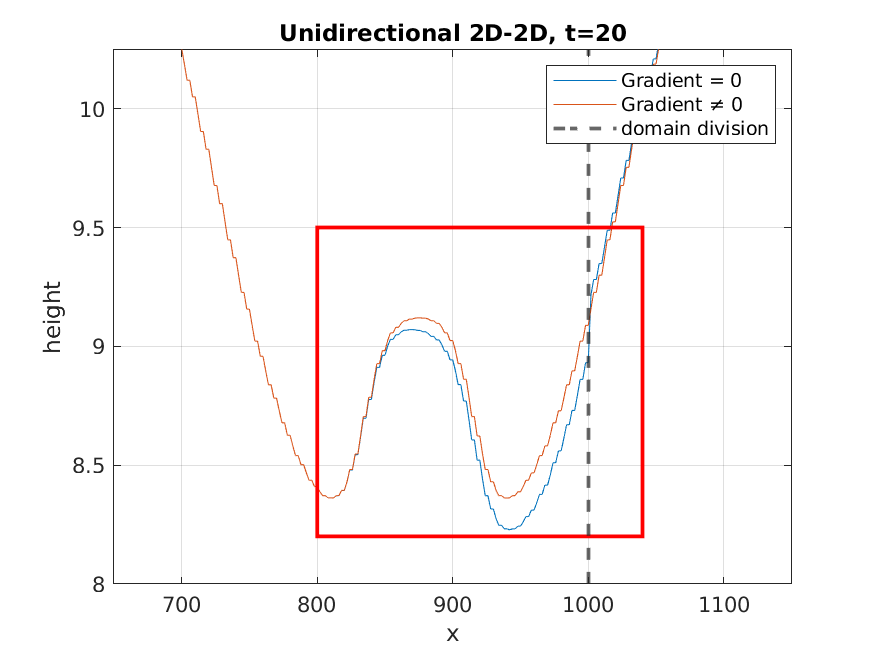
\includegraphics[width=.4\textwidth]{./Resources/Images/unidirectional_graph.png}
%
%\caption{Top right: $h(t=0)$. Left: $h(t=20), \nabla_\eta=0$. Middle: $h(t=20),\nabla_\eta \neq0$. Right: graphed values at the middle of the domain}
%\end{figure}

\end{frame}


%%%%%%%%%%%%%%%%%%
%%%%%%%%%%%%%%%%%%
%\begin{frame}
%\shiftedframetitle{Current Status}
%\vspace{-0.5cm}
%{\large $2D$ SWE - $2D$ SWE \textbf{\myTUMdarkblue{Bidirectional}}}\\
%Case: Radial dam break, no bathymetry
%\begin{textblock*}{1cm}(17cm,1pt) % {block width} (coords)
%%\begin{figure}
%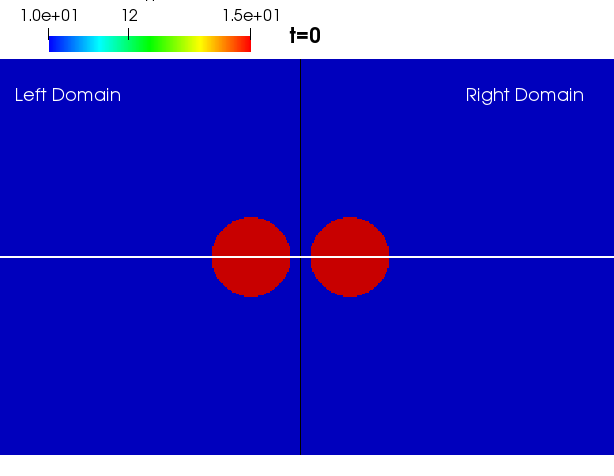
\includegraphics[scale=0.22]{./Resources/Images/bidirectional0_g_0.png}
%%\caption{sadf}
%%\end{figure}
%\end{textblock*}
%
%\begin{figure}[htp]
%\centering
%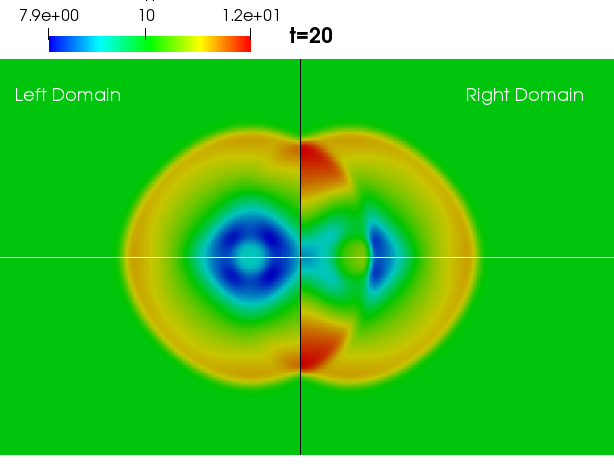
\includegraphics[width=.25\textwidth]{./Resources/Images/bidirectional20_g_0.png}\hfill
%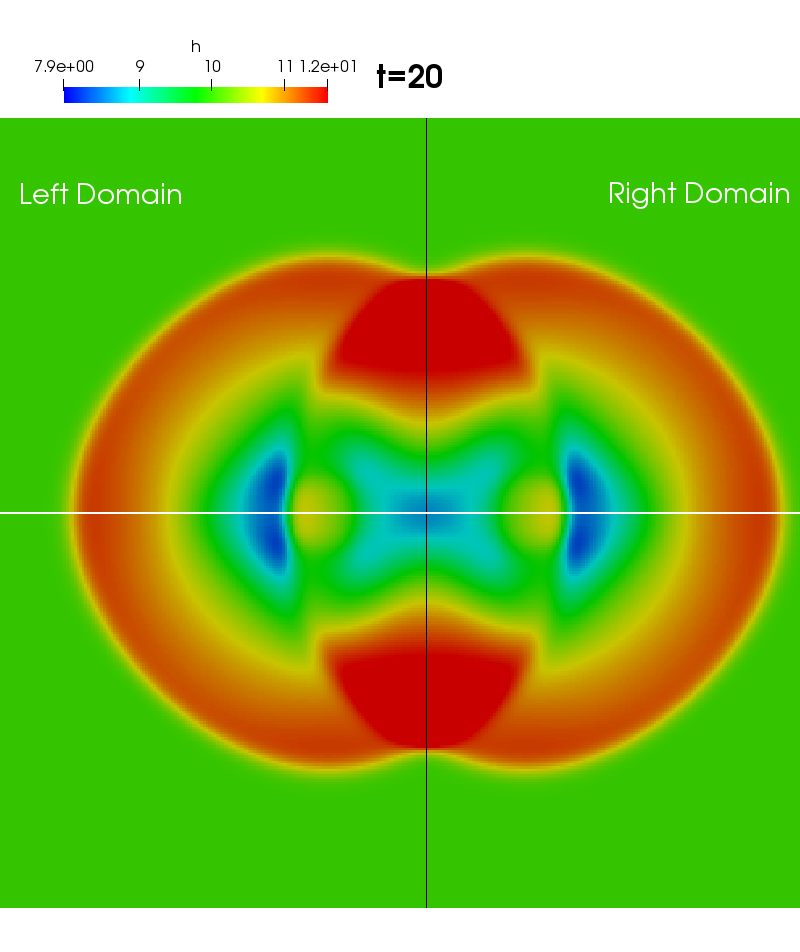
\includegraphics[width=.25\textwidth]{./Resources/Images/bidirectional20_g_bueno.png}\hfill
%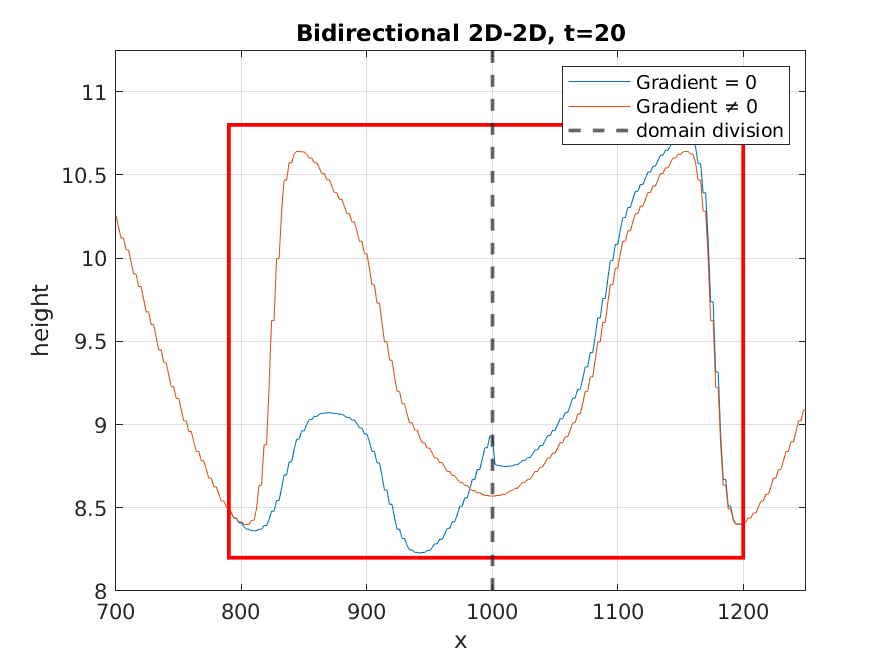
\includegraphics[width=.4\textwidth]{./Resources/Images/bidirectional_graph.png}
%\caption{Top right: $h(t=0)$. Left: $h(t=20),\nabla_\eta=0$. Middle: $h(t=20)$,$\nabla_\eta \neq0$. Right: graphed values at the middle of the domain}
%\end{figure}
%
%\end{frame}

